\section{Operativ systemet}

\begin{figure}[h!]
	\centering
	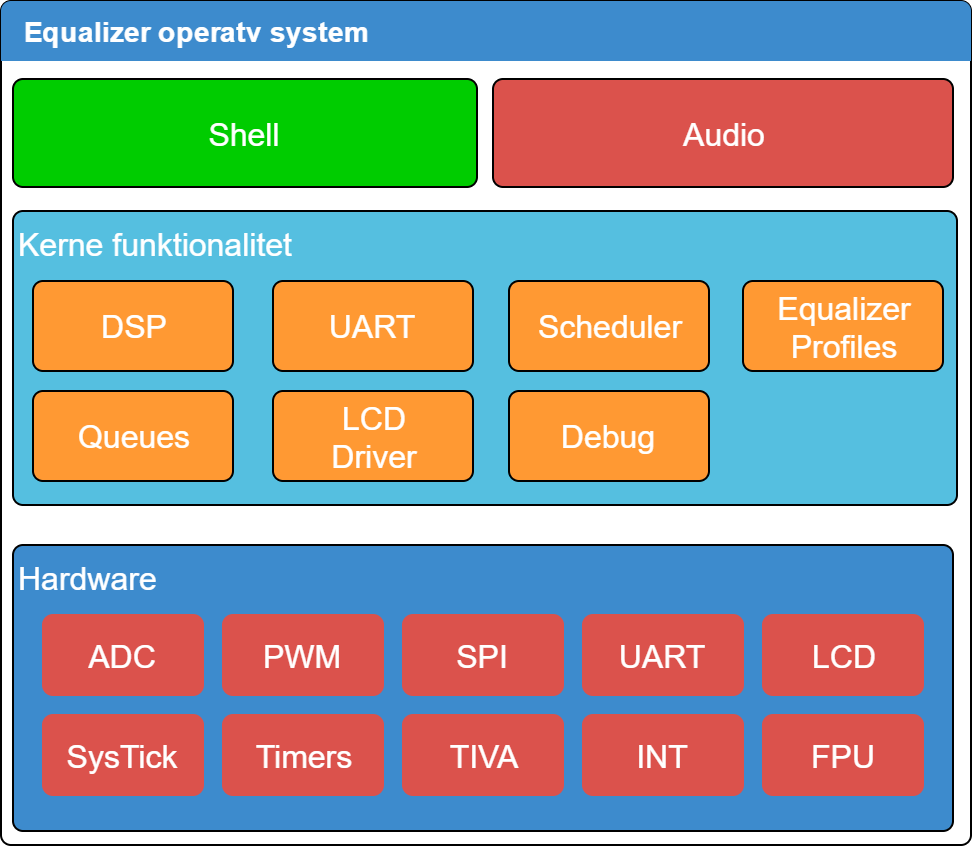
\includegraphics[width=.5\textwidth]{billeder/eq_os.png}
	\caption{Arkitektur af equalizerens operativ system.}
	\label{fig:eq_os}
\end{figure}

For at kunne håndtere de forskellige opgaver der kræves af equalizerens software, er det valgt at opbygge er simpelt operativt system.
Operativsystemet stiller funktionalitet til rådighed, som gør signalbehandling, kommunikation med brugeren igennem en shell og visning af information i et LCD display lettere at implementere. En oversigt over den valgte arkitektur kan ses i figur \ref{fig:eq_os}.\\

I det nederste lag findes den hardware specifikke funktionalitet, som primært består i opsætning og konfiguration af den valgte MCUs periferienheder, som f.eks. ADC, SPI, UART etc.\\
 
Ovenpå hardware laget, findes et udvalg af kernefunktionaliteter til at servicere systemet.
\begin{itemize}[noitemsep]
	\item UART til seriel kommunikation (SHELL).
	\item DSP funktionalitet til at lave beregninger for filtrere.
	\item Scheduler som sørger for at håndtere alle tasks for operativ systemet.
	\item Equalizer modul til at håndtere equalizer funktionalitet samt håndtering af profiler. 
\end{itemize}

Derudover er der servicemoduler som LCD driver, queues og debug funktionalitet.\\

I det øverste lag findes brugeradgangen til systemet, i form af en shell der kan benyttes via seriel kommunikation.
Signal behandlingen er ligeledes lagt på dette niveau, da lyden godt kan anses for at være den vigtigste \textit{"bruger"} af systemet.\\

Selv om systemet kan fremstilles som en lagdelt model, vil den nok mest kunne beskrives til at have en monolitisk struktur.
Dette skyldes at funktionalitet er meget tæt koblet.
Der er i designet og udviklingen ikke valgt at bruge et mere standardliseret indlejret operativ system som f.eks. freeRTOS eller lignende.
Hele systemet er opbygget løbende i udviklingsforløbet og sideløbende med undervisningsforløbet i embedded programmering.  

\FloatBlock